\chapter*{M2: Virtual Memory}{\textbf{Author: Chenyi Wang}
\newline
 \newline
 The goal of this milestone is to enable user-level processes to manage their virtual address spaces.}
\addcontentsline{toc}{chapter}{M2: Virtual Memory}
\section{Architecture Overview}
\subsection{Page table representation}

We keep a software shadow tree of the hardware page tables so we can find any
mapping by virtual address without re-walking the live tables. The data
structure is struct \co{shadow_pt} in \co{include/aos/paging_types.h}, one node per
hardware L0/L1/L2/L3 table, carrying the capref of that vnode, the mapping
cap that installed it into its parent, and a 512-entry children array
indexed by the same PTE slot that the hardware would use. The L0 root
is at \co{paging_state.l0_shadow} and is built in \co{paging_init_state}. Levels
below it are created lazily by \co{ensure_l3} the first time a mapping touches
that subtree. We never pre-allocate a level we have not used.

\medskip\noindent
This mirror is what makes unmap and shadow tree walks cheap. Without it we
would either have to traverse the kernel page tables through the cap system,
which is not part of the user-side API, or remember every pair in a list, which scales poorly.

\medskip\noindent
Looking ahead, we could use a balanced shadow tree to make lookups easier. Another
advantage of the shadow tree is that it would let us support superpages. A leaf
node could attach directly at the L0/L1/L2 level of the tree, depending on how
large the superpage is. This feature would be hard to support with other data
structures.

\subsection{Virtual address space tracking}

The free and allocated VA regions live in a single sorted doubly linked list
of struct \co{vregion}, rooted at \co{paging_state.vregions}. Each
node carries base, size, an allocated flag, and pointers to its neighbors.
On init the list contains one big free region from \co{start_vaddr} to
\co{MAX_VA_ADDR}, which is 0x7f.

\medskip\noindent
\co{paging_alloc} walks the list, picks the first free node large enough, splits
off the wasted front for alignment using \co{vr_split_front} and splits off any
excess at the back using \co{vr_split_back}, then marks the result allocated.
\co{paging_unmap} reverses the process. It clears the runs, marks the vregion free,
then coalesces with the previous and next neighbors if they are also free.
\co{vr_coalesce} is the only place that drops nodes back to the slab. The list
is kept sorted by base address as an invariant of the splits, which is what
lets us walk it forwards and find any address in O(N).

\medskip\noindent
We chose a linked list over a balanced tree because the working set of
vregions is small in practice and the constant factor on a tree node was not worth
the extra slab pressure. If a future workload pushes the list into the
thousands we would switch to a red-black tree without changing any caller.

\subsection{Map and unmap}

\co{paging_map_frame_attr_offset} is the workhorse. It ensures the helper slabs
have room, possibly triggers a root cnode refill, calls \co{paging_alloc} to
reserve VA, then calls \co{do_map} to install the PTEs.

\medskip\noindent
\co{do_map} chunks the requested region at L3 boundaries and
issues one \co{vnode_map} per chunk. For each chunk it records a \co{vregion_run}
holding the L3 shadow node, the starting slot, the page count, and the
mapping cap. The runs form a per-vregion list rooted at \co{vregion.runs}.
Recording the chunks instead of synthesizing them later is what makes
\co{paging_unmap} simple. It walks \co{vregion.runs}, calls \co{vnode_unmap} plus
\co{cap_destroy} per run, frees the run nodes back to the slab, and is done.
The unmap path never re-walks the shadow tree.

\medskip\noindent
\co{paging_map_fixed_attr_offset} shares \co{do_map} and the run tracking. It
adds a containment check, finding the unique free vregion that fully contains
\co{[vaddr, vaddr+bytes)}, rejecting the request if the range overlaps any allocated
region, and otherwise carving and installing. This is the path that V02 and V05
stress with their overlap-rejection requirements.

\subsection{Lazy Heap Allocation}

\co{morecore_alloc} only reserves virtual address space; it never touches a
physical frame. The implementation in \co{lib/aos/morecore.c}
calls \co{paging_alloc} with the requested size and returns the base address. The cost of a malloc is O(1)
in the number of pages, independent of how big the allocation is. The book
suggested implementing eager mapping first and switching to lazy later. We
implemented lazy from the start because the work to back up an unmapped
heap with a page fault handler was already required for the grading tests,
and bolting eager mapping on top would have been throwaway code.

\medskip\noindent
\co{morecore_free} walks the vregion list to find the region that contains the
freed pointer, then calls \co{paging_unmap} on its base address. This means the
full VA region returns to the free pool in one shot, which is fine because
malloc and free always pair on the same vregion base address.

\medskip\noindent
The lazy design has the consequence that any heap miss inside the bench
harness shows up as a page fault, not as a malloc cost. This is exactly the
property that MB3 in our benchmark relies on.

\subsection{Page Fault Handler}

\co{pagefault_handler} in \co{lib/aos/paging.c} is registered via
\co{set_main_handler} for the main thread and via \co{paging_init_onthread}
for each additional thread. The handler is small on purpose. It rejects any
fault at an address below \co{NULL_GUARD_ADDR} = 32 MiB as a null dereference,
walks the vregion list to find the allocated region that owns the faulting
page, makes sure the helper slabs have room, allocates one \co{BASE_PAGE_SIZE}
frame, builds the L3 shadow node via \co{ensure_l3} if it does not exist yet,
and installs exactly one PTE through \co{vnode_map}. The new run is pushed onto
the \co{vregion.runs} list so \co{paging_unmap} can find it later.

\medskip\noindent
Two non-obvious decisions shape the handler. First, the PTE is installed
directly rather than through the standard map path:
\co{paging_map_fixed_attr_offset} rejects already-allocated vregions, which
would cause the fault to loop forever. Second, all three \co{ensure_X_slab}
calls run before \co{frame_alloc} so the handler never recurses into itself
by faulting during a slab refill.

\subsection{Slab Allocators}

We carry three slabs in struct \co{paging_state} --- \co{pt_slab} for \co{shadow_pt}
nodes, \co{vr_slab} for \co{vregion} nodes, and \co{run_slab} for \co{vregion_run} nodes.
Each is sized differently because \co{shadow_pt} is roughly 4 KiB while \co{vregion}
and \co{vregion_run} are small. The initial paging state is seeded from three
file-static buffers, so the very first allocations never have to go through the
slab refill path that itself needs paging.

\medskip\noindent
Once those static buffers are warm, the slabs grow on demand through dedicated
refill functions: \co{ensure_vr_slab}, \co{ensure_run_slab}, and
\co{ensure_pt_slab}. Each calls
\co{slab_refill_no_pagefault}, which allocates a frame and maps it through
\co{paging_map_frame_attr}. The three \co{ensure_X_slab} functions share a
re-entrancy guard pattern: any one of them being mid-refill blocks the others
from refilling too. This is required because \co{slab_refill_no_pagefault}
calls back into \co{paging_map_frame_attr_offset}, which would otherwise drive
each of the other two slabs to refill recursively before the outer one finishes.

\subsection{Slot Allocator Refill}

\co{paging_map_frame_attr_offset} and \co{paging_map_fixed_attr_offset} both
peek at the single slot allocator state before they reserve a vregion. If
the root cnode is down to twelve free slots, the map path triggers a manual
\co{root_slot_allocator_refill} guarded by the state \co{rootca.refilling}
so the refill path does not re-enter itself. The threshold of twelve was
picked empirically. A single map request can chew through several slots, so
we want headroom before the slot allocator itself starts demanding new slots
from the root.

\subsection{Limitations and follow-ups}

The vregion free list is a plain linked list with linear time alloc and
linear time fault handler lookup. Under heavy fragmentation this becomes
the bottleneck; a balanced tree would fix it without changing callers.

\medskip\noindent
Superpages are not implemented. \co{do_map} only emits \co{BASE_PAGE_SIZE} PTEs, so
the flag is silently dropped. Hooking 2 MiB block PTE installation into \co{do_map}
is the next planned extension and would also enable the MB5 superpage comparison
in our benchmark plan.

\section{Evaluation}

We evaluate the M2 paging subsystem with a VM PUP-style microbenchmark
modelled on Appel and Li's 1991 ASPLOS paper. All numbers below are from
a single run on the imx8x board with the system counter at 8\,MHz. Each
result row is emitted as a CSV line and post-processed into the plots
that follow. The reservation size used in the lazy/eager and hybrid
experiments is fixed at 1000 pages.

\subsection{Base costs}

We start with the four primitive cost numbers, shown in
Figure~\ref{fig:m2bench}. The leftmost two columns are language-level
baselines, a register-to-register integer add and a write to an
already mapped page. The rightmost two are the headline VM operations,
mapping then unmapping a single page and faulting in a single page
through the user-mode page fault handler.

\begin{figure}[h]
    \centering
    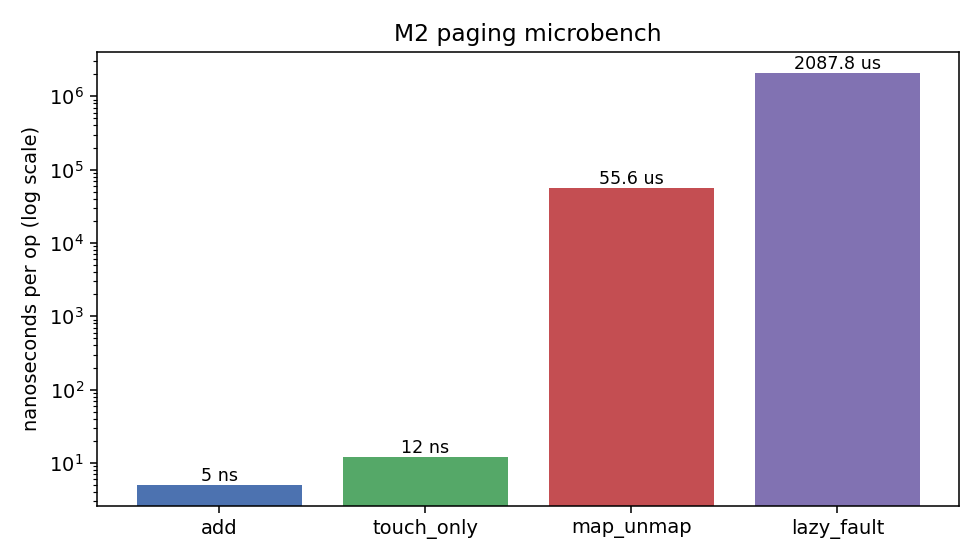
\includegraphics[width=0.85\textwidth]{fig/m2_bench.png}
    \caption{Per operation cost of the four primitives. Log scale on the y
    axis; the four bars span roughly six orders of magnitude.}
    \label{fig:m2bench}
\end{figure}

\noindent
A bare add costs five nanoseconds and a touch on an already mapped page
twelve nanoseconds, so the cost of installing a single page table entry
under our paging code, including the explicit unmap, is around four
orders of magnitude above the bare arithmetic baseline. A single
user-mode page fault is another factor of forty on top of that. This
gap is exactly the phenomenon Appel and Li raised in 1991, and we
revisit it below in the historical comparison.

\subsection{Comparison to 1991 systems}

Figure~\ref{fig:m2_appel_li} compares our user-mode page fault round
trip to the seven systems Appel and Li tabulated in 1991. The left
panel reports absolute wall clock time, the right panel reports the
same number divided by each system's own add cost, which is the
normalization Appel and Li argued for. Our results make their argument
even stronger.

\begin{figure}[h]
    \centering
    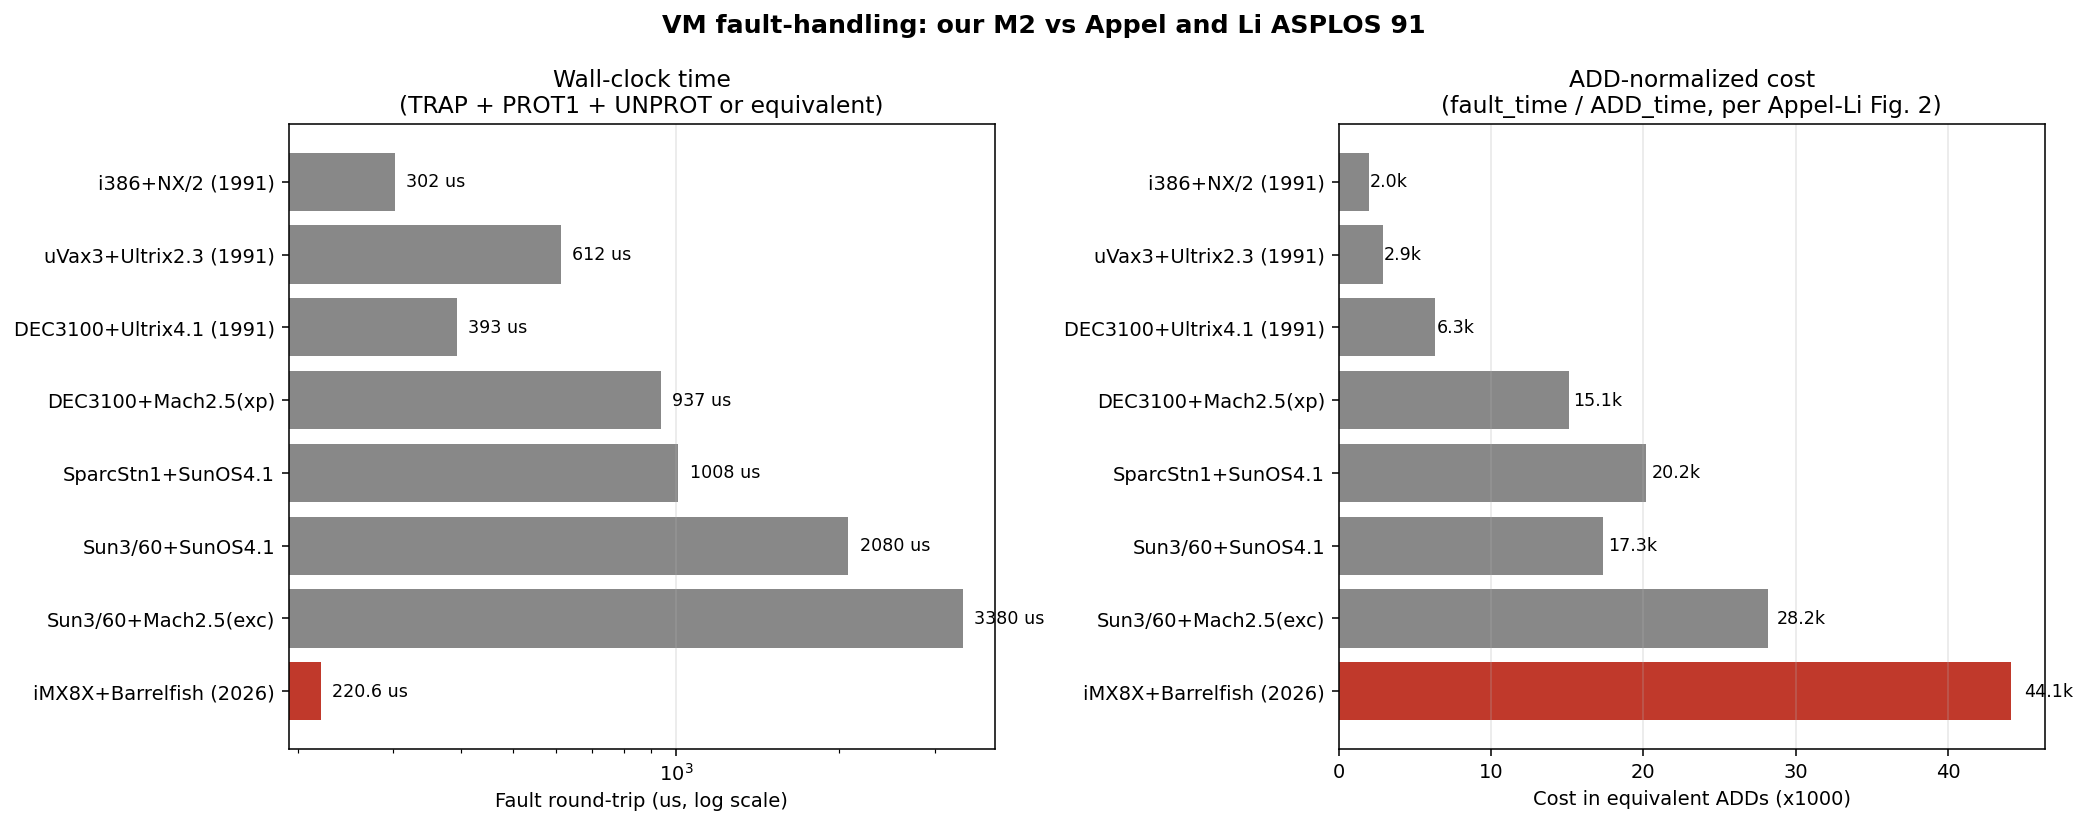
\includegraphics[width=\textwidth]{fig/m2_vs_appel_li.png}
    \caption{Page fault round trip on our system against the seven 1991
    systems tabulated in Appel and Li's paper.}
    \label{fig:m2_appel_li}
\end{figure}

\noindent
In absolute time we are the fastest of the comparison set, at 220
microseconds against a 1991 range of 300 microseconds to 3.3
milliseconds. Once we normalize by add cost, the picture inverts. Our
fault costs about forty-four thousand adds, against a 1991 range of
two thousand to twenty-eight thousand. CPUs have gained roughly three
orders of magnitude in the intervening decades but our VM round trip
has only halved, so the relative cost of a fault has actually grown.
The complaint Appel and Li levelled in 1991 still applies, only more
so. The cost of crossing into the kernel and back, even on a modern
ARMv8 with a user-mode page fault handler that we wrote ourselves, has
not kept up with the rest of the machine.

\subsection{Allocation Strategies Across ``Touch Ratios''}

For the comparison between lazy and eager allocation we vary the
fraction of the reserved region that is actually touched, from ten
percent up to one hundred percent in steps of ten.
Figure~\ref{fig:m2_lve_sweep} shows both panels, physical frames
committed on the left, total wall clock time on the right.

\begin{figure}[h]
    \centering
    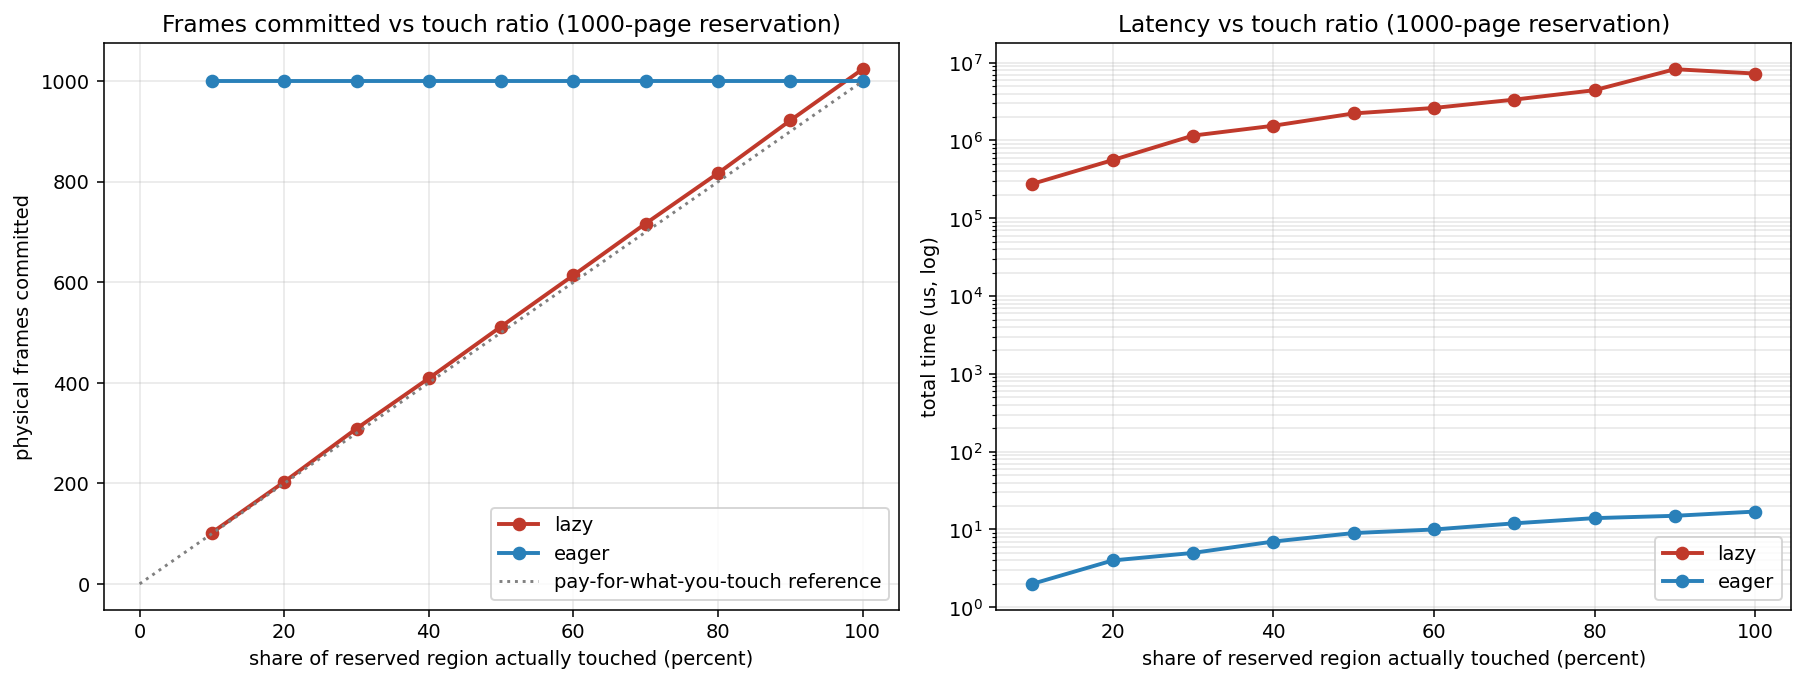
\includegraphics[width=\textwidth]{fig/m2_lve_sweep.png}
    \caption{Lazy versus eager as the touched fraction of the
    reservation grows. Reservation is 1000 pages throughout.}
    \label{fig:m2_lve_sweep}
\end{figure}

\noindent
The frame plot reproduces the obvious story very cleanly. Lazy tracks
the diagonal, committing one frame for each page that is actually
touched, plus a small constant overhead from the slab allocator and
the page fault path itself. Eager sits flat at one thousand frames
regardless of how many of them get used, because the reservation is
satisfied by a single batch map up front. At a ten percent touch
ratio, eager is committing ten times more physical memory than the
workload actually requires.

\medskip\noindent
The time plot is the corresponding cost. Eager stays in the low tens
of microseconds across the entire sweep, dominated by the one-shot
batch map. Lazy starts at about 280 milliseconds for one hundred
faults and grows roughly linearly with the number of faulted pages,
reaching seven seconds at one thousand pages. The two curves never
cross. As long as we are willing to pay for physical memory up front,
eager is two to five orders of magnitude faster than lazy on this
hardware.

\subsection{Hybrid Strategy Under Random Access}

The natural next question is whether a strategy that pre-maps some of
the reservation eagerly and lets the rest fault in lazily can beat
either endpoint. Pre-mapping costs memory but eliminates faults on
hits, so the answer depends on what fraction of the touches hit the
pre-mapped pages.

\medskip\noindent
To stay honest we drive this experiment with a random access pattern. The
bench seeds the C library random number generator from the system counter
and issues each touch at a uniformly random index over the whole
reservation, so the access pattern carries no oracle information about
which pages will turn out to be hot. A touch falls in the pre-mapped region
with probability proportional to the size of that region, and hits the lazy
region the rest of the time.

\medskip\noindent
Figure~\ref{fig:m2_hybrid} sweeps the preload region size across 0\% to
100\%, touching 100 random pages in each run. The two dashed reference
lines are pure lazy and pure eager at the same touch count.

\begin{figure}[h]
    \centering
    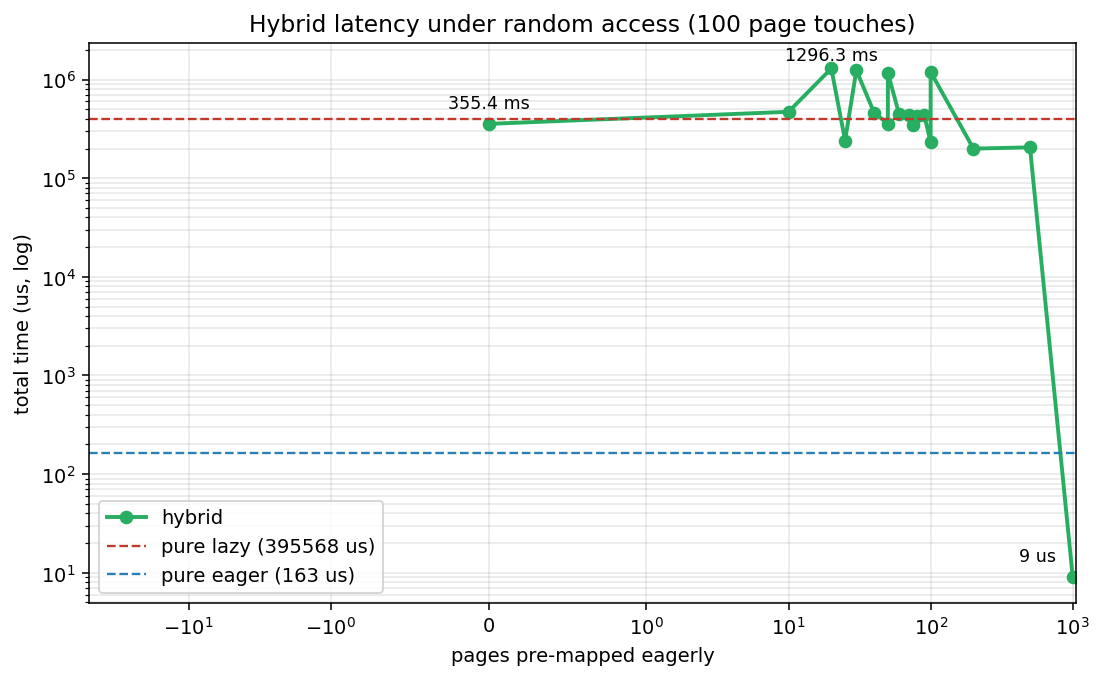
\includegraphics[width=0.85\textwidth]{fig/m2_hybrid.png}
    \caption{Hybrid latency as the eager region grows from zero to the
    full reservation. Random touch pattern, 100 touches.}
    \label{fig:m2_hybrid}
\end{figure}

\noindent
The curve sits within a factor of three of the pure lazy reference for
every intermediate size we tested. Even with five hundred pages
pre-mapped, the wall clock time only drops to about 200 milliseconds,
against pure lazy's 355 milliseconds. The cliff that finally takes the
line down to nine microseconds appears only at the right edge of the
sweep, where the eager region equals the full reservation and there is
no lazy region to fault into. In other words, on random access the
hybrid policy degenerates. Unless you pre-map essentially everything you
might touch, the touches that miss the pre-mapped region still pay the
full per-fault cost, and the small expected number of hits is not enough
to move the total.

\medskip\noindent
The narrow sweep in Figure~\ref{fig:m2_hybrid_mix} zooms into the
region where the pre-mapped size and the touch count match, varying
the eager region from ten to one hundred pages.

\begin{figure}[h]
    \centering
    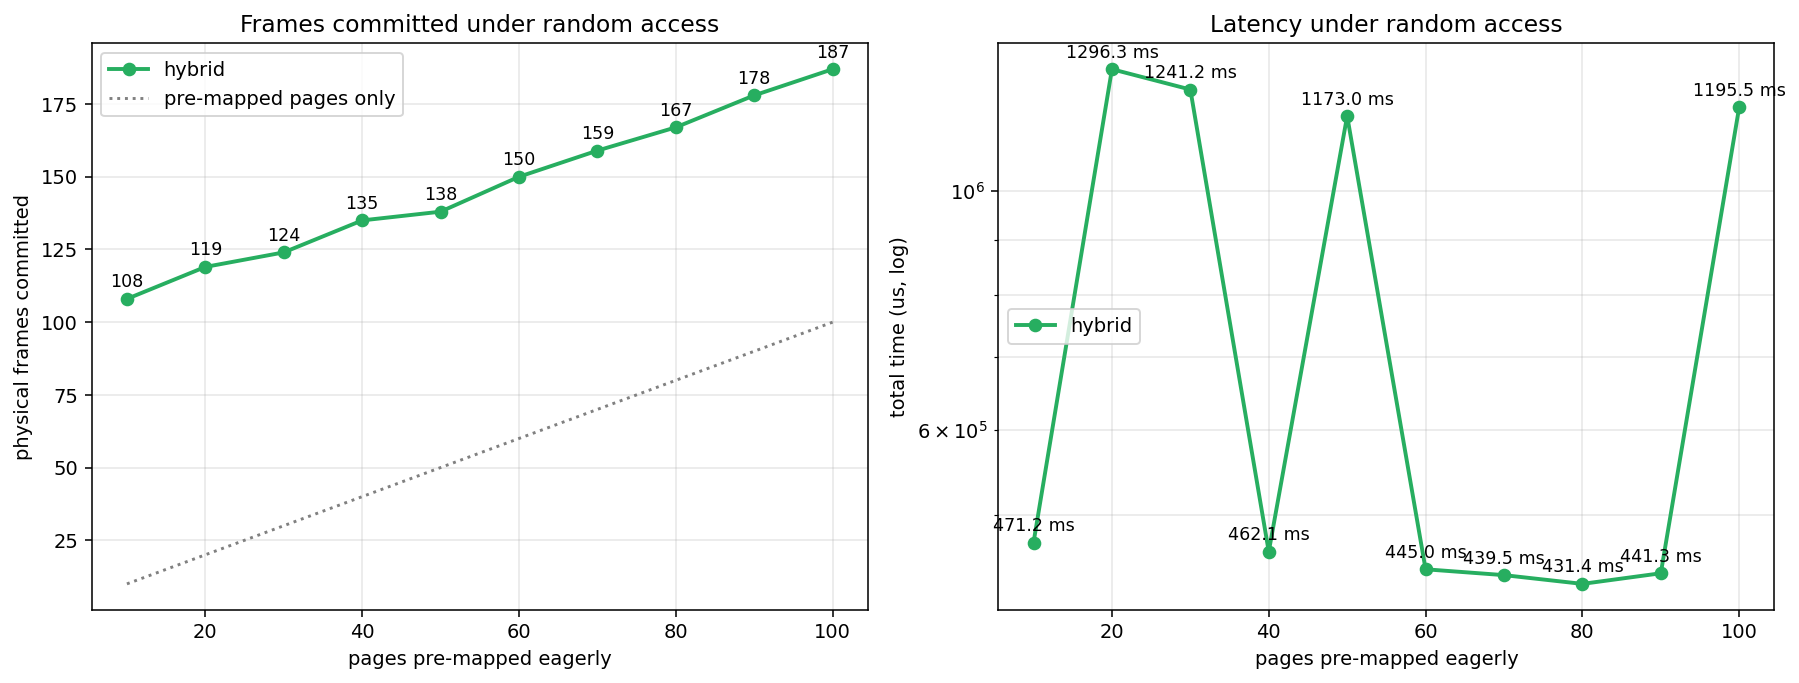
\includegraphics[width=\textwidth]{fig/m2_hybrid_mix.png}
    \caption{Hybrid frames and latency for small eager regions, with
    a fixed 100 touch random workload over a 1000 page reservation.}
    \label{fig:m2_hybrid_mix}
\end{figure}

\noindent
The frame panel grows monotonically from 108 to 187, well above the
grey reference line that shows what the pre-mapped pages alone would
cost. The gap between the curve and the reference is the lazy region's
contribution, since roughly nine out of ten random touches still miss the
pre-mapped region and bring in a fresh frame. The latency panel is
noisy enough that we treat the individual points with caution; the
average sits around 700 milliseconds and shows no clean trend across
the sweep. The committed frame count grows by about ten pages for each
ten-page increase in the pre-mapped region, but the time stays in the
same band as pure lazy.

\subsection{Frames Versus Time Trade-off}

Figure~\ref{fig:m2_mem} brings the three strategies onto a single
trade-off plot. The bar chart on the left shows physical frames
committed at a hundred-touch workload, with the hybrid case shown for
three representative pre-map sizes. The scatter on the right places
each strategy in the two-dimensional space of memory cost versus time
cost.

\begin{figure}[h]
    \centering
    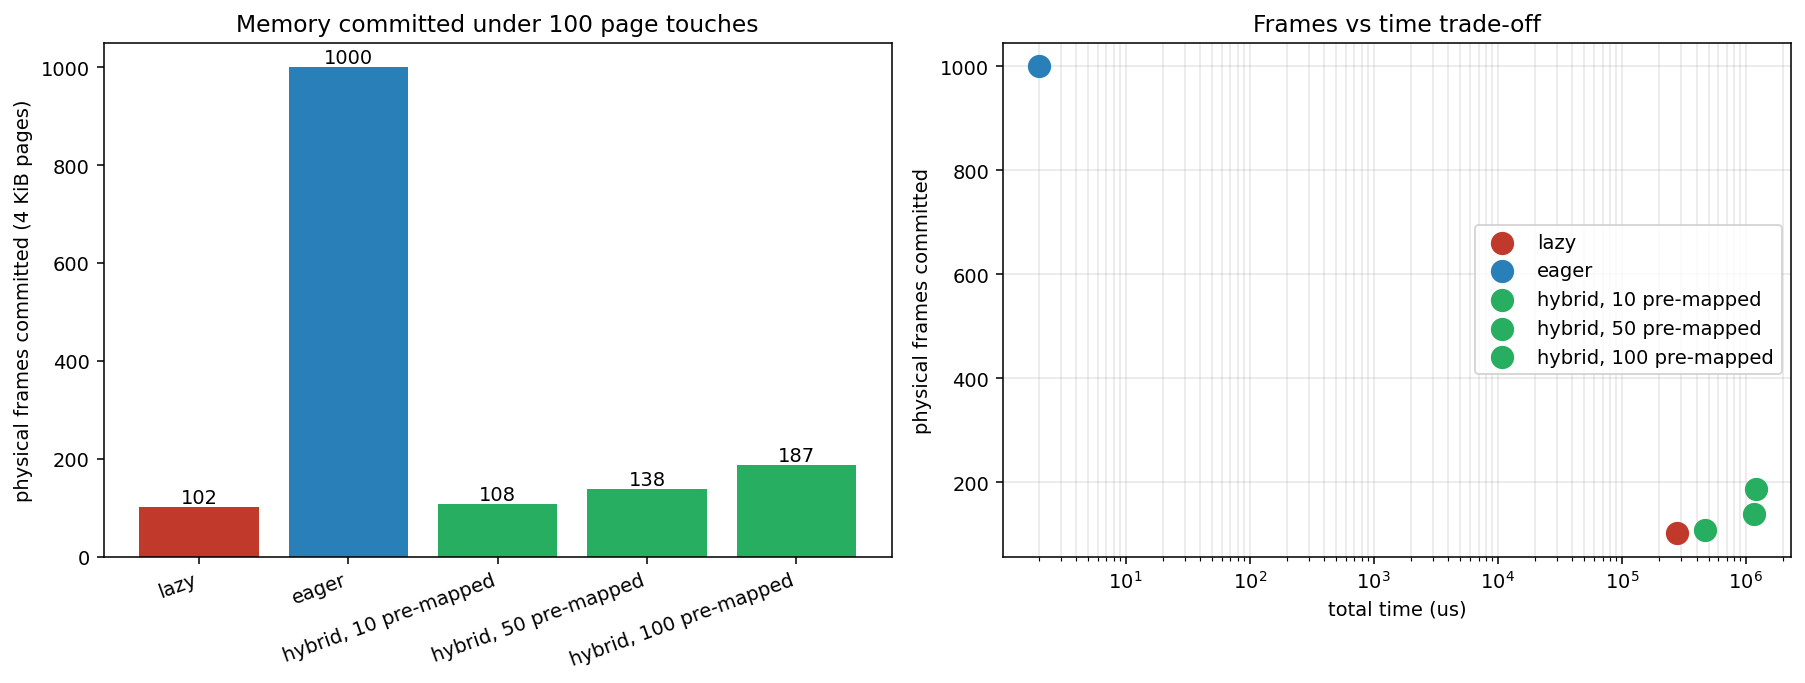
\includegraphics[width=\textwidth]{fig/m2_mem.png}
    \caption{Eager pays ten times the memory for
    near zero touch latency; lazy and hybrid land in the same lower
    band of memory but pay hundreds of milliseconds.}
    \label{fig:m2_mem}
\end{figure}

\noindent
Eager sits alone in the upper left of the scatter, which means it
commits the full thousand frames but the touches themselves take only
two microseconds because every PTE is already installed. Lazy and the
three hybrid points cluster in the lower right, all at roughly one
hundred to two hundred frames and all at hundreds of milliseconds of
wall clock time. Lazy is the best of that cluster, committing the
fewest frames and running in the shortest time of any non-eager option.
None of the hybrid points dominate it on either axis.

\medskip\noindent
The practical conclusion for our system is that there are two
sensible policies and no useful middle ground. If memory pressure is
the binding constraint, lazy is the right choice; the per-fault
cost is high but the physical commit is exactly what the workload
uses. If latency is the binding constraint and the reservation can be
fully committed up front, eager wins by four orders of magnitude
because it amortizes the per-page cost into a single batch map.
Hybrid is dominated by lazy in the random-access regime we measured.
It would only become attractive if the access pattern were known in
advance, in which case the pre-mapped region could be sized to cover
exactly the hot pages and the experiment would collapse back into a
small eager allocation.
\newpage
\section{Development Process}
For this milestone, Allan began by defining all the relevant data 
structures for the page tables. \co{include/aos/paging_types.h} contains
all the definitions for the shadow page tables, the virtual memory \co{vregion}s,
and the extensions which allow us to map a frame into multiple L3 page tables.
Then he also implemented the paging code to map frames into these newly created
structures in \co{lib/aos/paging.c}.

\medskip\noindent
Sahil then implemented the unmap code as well as the other paging function. 
To finish up the pre-testing code, Shane implemented the \co{morecore} code 
as well as working on the lazy allocator with the page fault handler.

\medskip\noindent
The main challenge we faced with this milestone was probably refilling the slabs.
We cannot refill the slabs when we completely exhaust the pools, as the refill
code requires the paging code which has exhausted slabs. So we decided on a 
threshold, which eventually allowed us to pass the milestone.
